%%%%%%%%%%%%%%%%%%%%%%%%%%%%%%%%%%%%%%%%%%%%%%%%%%%%%%%%%%%%%%%%%%%%%%%%%%%%%%%%
% app-exp-setup.tex: Experimental setup description.
% behavior
%%%%%%%%%%%%%%%%%%%%%%%%%%%%%%%%%%%%%%%%%%%%%%%%%%%%%%%%%%%%%%%%%%%%%%%%%%%%%%%%
\chapter{Experimental Setup}\label{app:exp-setup}

We use the ARGoS simulator~\cite{Pinciroli2012} with a dynamical physics model of
the marXbot (\cite{Dorigo2005c}) in a 3D space for maximum fidelity (robots are
still restricted to motion in the XY plane).

\section{Foraging Task Decomposition Graph}\label{sec:exp-foraging-tdgraph}

We instantiate the task decomposition graph shown in Fig.~\ref{fig:tdgraph-foraging},
extending previous work~\cite{Harwell2018,Pini2011b,Ferrante2015} which explicitly or
implicitly defined the following tasks, implemented as vertices comprising
$\TAGraphV{a}$ (gold vertices in Fig.~\ref{fig:tdgraph-foraging}):
%
\begin{figure}[!htbp]
  \centering
  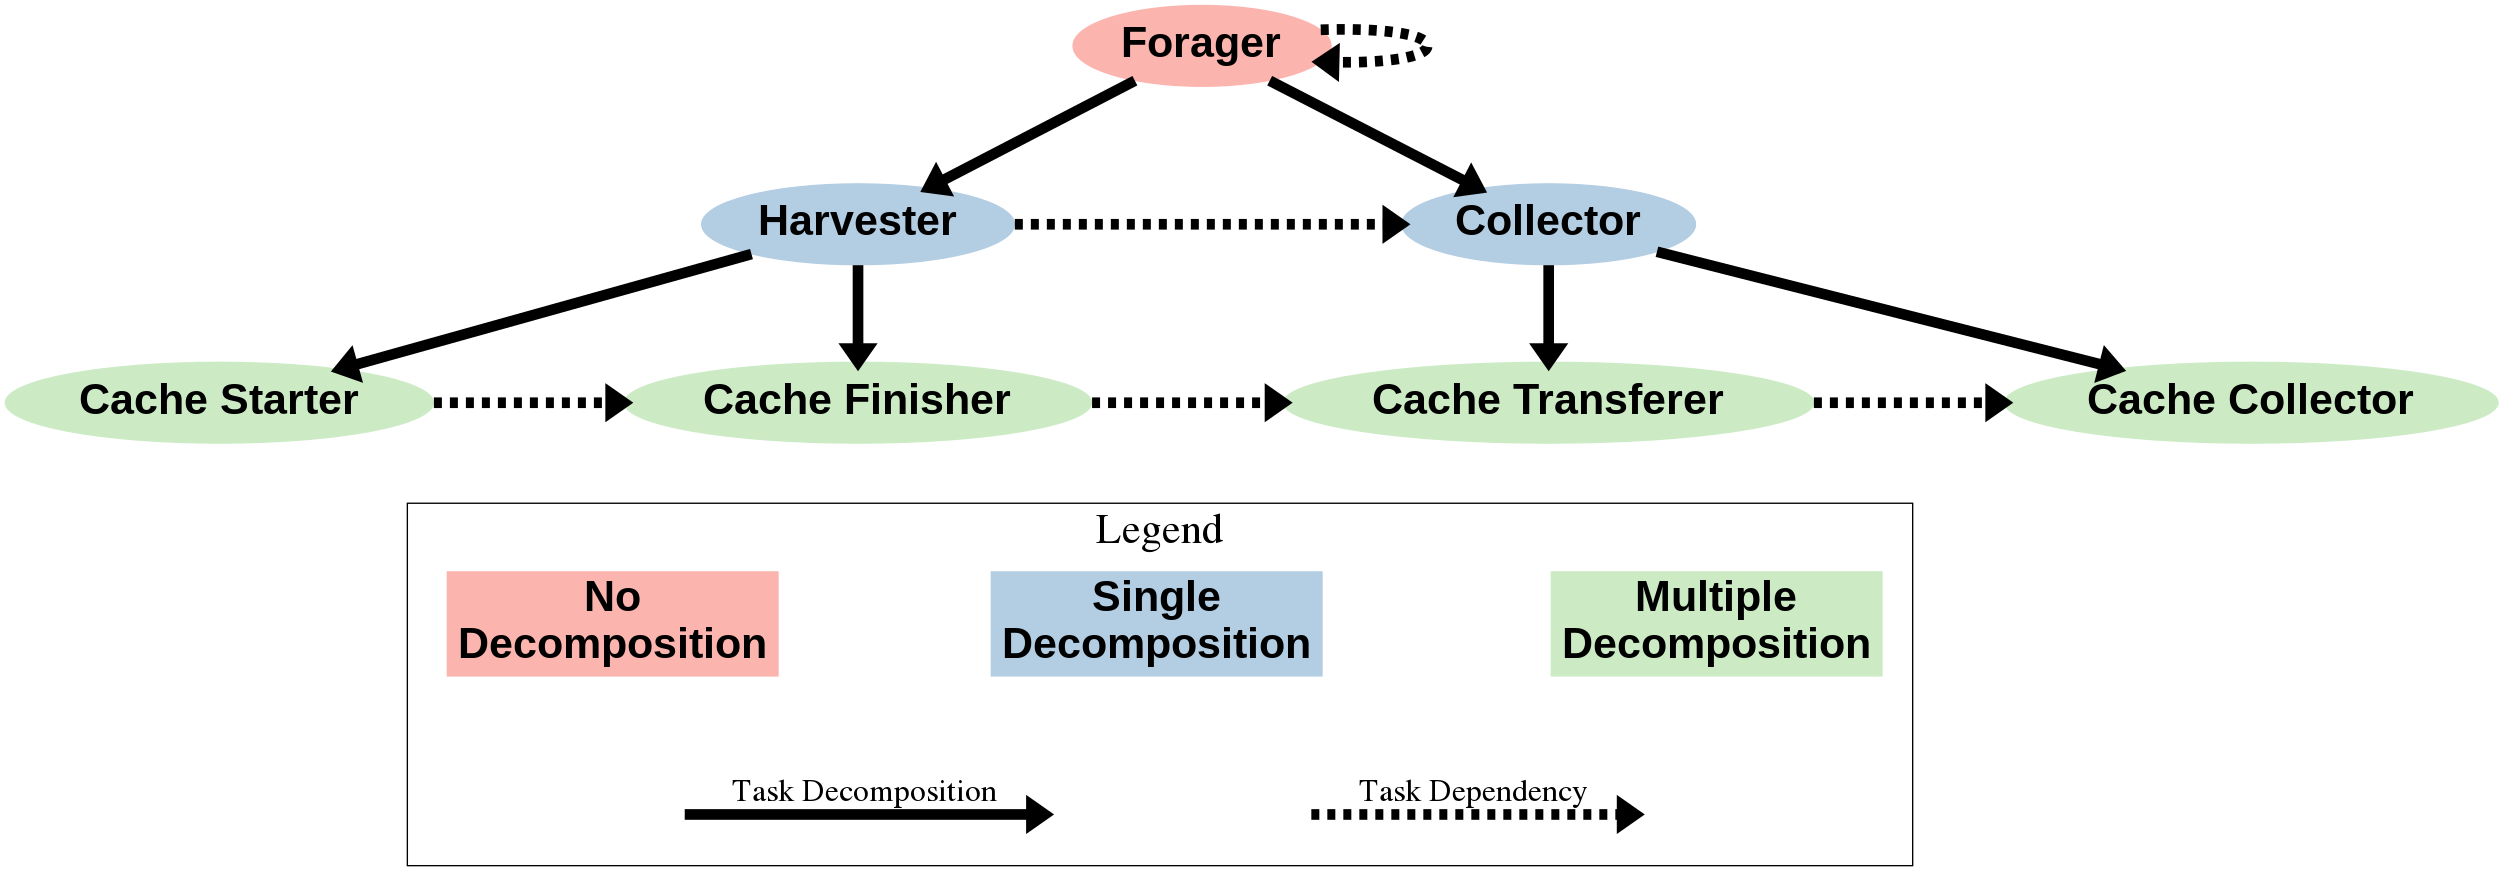
\includegraphics[width=\textwidth]{figures/chapter2/tdgraph-foraging.png}
  \caption[Task decomposition graph, $\TDGraph$, for a foraging
  task, in which robots have to
   find spatially distributed objects in the environment and then bring them to
   a central location.]{\label{fig:tdgraph-foraging}
   Red+blue tasks correspond to a scheme in which robots do
   a whole task or 1/2 task (single decomposition option).  Red+blue+green tasks
   correspond to a scheme in which robots do a whole task, 1/2 task, or 1/4 task
   (multi-decomposition option).  However, by choosing to decompose the task
   into multiple parts, there now exist task dependencies between the parts,
   which the swarm has to collectively learn to be successful.
   Blue tasks ($\phi_i=1$) were defined in~\cite{Harwell2018}, green tasks
   ($\phi_i=2$) were defined~\cite{Harwell2019a}.}
\end{figure}

\begin{itemize}
\item \emph{Forager}: Acquire a free block of highest utility and bring it to the
  nest. This is $\TAGraphRoot$, and one way of accomplishing the swarm objective
  $\SwarmObjective$ via $\phi_0$.

\item \emph{Harvester}: Acquire a free block of highest utility and bring it to the
  existing cache of highest utility, calculated as:
%
  \begin{equation}\label{eqn:existing-cache-utility}
    \mu_{\hat{C_j}}(t) = \frac{e^{-\tau_{\hat{C_j}}(t)}{\lvert \hat{C_j} \rvert}}{\norm{\ArbRobot - \mathbf{C_j}}\norm{\mathbf{C_j} - \mathbf{nest}}}
  \end{equation}
%
  where $\lvert \hat{C_j} \rvert$ is the estimated size of the $j$th cache known to
  $\ArbRobot$ (caches might not exist anymore, and therefore a robot only has
  estimates of their existence). This equation emphasizes selection of caches that
  are close to the position of $\ArbRobot$, but also that are closer to the nest,
  while accounting for the relevancy of a robot's information about
  $C_j$~\cite{Harwell2018}. This task accomplishes part of $\SwarmObjective$ via
  $\phi_1$.

\item \emph{Collector} Acquire a block from the existing cache of highest utility
  (Eqn.~\eqref{eqn:existing-cache-utility}) and bring it to the nest. This task
  accomplishes part of $\SwarmObjective$ via $\phi_1$.
\end{itemize}
%
We extend prior work with the following tasks, implemented as vertices comprising the
task sequence $\phi_2$ (red vertices in Fig.~\ref{fig:tdgraph-foraging}):

\begin{itemize}
\item {\emph{Cache Starter}: Acquire a free block of highest utility and bring it
    partway back to the nest, and then drop it at a feasible site to start a \emph{De
      Novo} cache, according to Eqn.~\eqref{eqn:cache-site-select}. A feasible site
    is one at least a distance $\eta$ from all known caches
    $\hat{C_1}\ldots\hat{C_n}$.
    %
    The best cache site \textbf{x} for $\ArbRobot$ is computed as follows:
    %
    \arraycolsep=0.75pt
    \begin{equation}
      \label{eqn:cache-site-select}
      \begin{array}{lc}
        \underset{\mathbf{x}}{\max} & \mu_{\ArbRobot} \\
        \text{s.t.} & \norm{\mathbf{x} - \mathbf{\hat{C_{m}}}} \geq \eta, \; m = 1, \ldots, n. \\
      \end{array}
    \end{equation}
    where
    \begin{equation}
      \label{eqn:cache-site-utility}
      \mu_{\ArbRobot} = {\Big(\norm{\mathbf{x} -\mathbf{x}_{\ArbRobot}} \norm{\mathbf{x} - \frac{\mathbf{x}_{\ArbRobot} - \mathbf{nest}}{2}}\Big)}^{-1} \\
    \end{equation}

    % [JRH] see if I can find some natural analogues of this sort of utility--would
    % really strengthen my choice of utility function
    Intuitively, cache sites that are close to $\mathbf{x}_{\ArbRobot}$ are better
    (less work to get to, less chance of being found unsuitable upon arrival), as are
    sites that are close to the halfway point between the robot's current position
    and the nest (bisecting the space maximizes available areas for \emph{Collector}
    and \emph{Harvester} tasks, reducing interference). This task accomplishes part
    of $\SwarmObjective$ via $\phi_2$.}

\item {\emph{Cache Finisher}: Acquire a free block of highest utility and place it
    within a distance $\eta$ to a \emph{De Novo} cache (a single free block a
    distance $\eta$ from all other blocks) of maximum utility
    (Eqn.~\eqref{eqn:existing-cache-utility} with $\lvert\hat{C_j}\rvert = 1$) in
    order to create a new cache. This task accomplishes part of $\SwarmObjective$ via
    $\phi_2$.}

\item {\emph{Cache Transferer}: Acquire a block from the existing cache of highest
    utility and transport it to the existing cache with the second highest
    utility. This accomplishes part of $\SwarmObjective$ via $\phi_2$.  }
\item {\emph{Cache Collector}: Acquire a block from the existing cache of highest
    utility (Eqn.~\eqref{eqn:existing-cache-utility}) and bring it to the nest. This
    task accomplishes part of $\SwarmObjective$ via $\phi_2$.}
\end{itemize}

By defining $\phi_2$, we have also implicitly defined $\beta_1,\beta_2$.

\section{Foraging Scenarios}\label{sec:exp-foraging-scenarios}

% [JRH] Show pictures of all the scenarios here, talk a little about each (e.g.,
% why PL is the most challenging scenario type).

\section{Source Code}\label{sec:exp-source-code}

% [JRH] Put a few bits about SIERRA/TITERRA in here.

Our open-source code is available at https://github.com/swarm-robotics/fordyca,
https://github.com/swarm-robotics/silicon,
https://github.com/swarm-robotics/sierra, and
https://github.com/swarm-robotics/titerra.
